%!TEX root = ../dissertation.tex

\chapter{Lo stage}
In questo capitolo vengono discussi i vari aspetti dello stage concernenti il processo di sviluppo.
Ciascuna attività di progetto viene analizzata e descritta nel dettaglio.


\begin{comment}
% Tabella da personalizzare in base alle ore delle attività
\begin{table}[]
\begin{tabular}{|c|c|}
	\hline
	    \rowcolor{blizzardblue}
	\textbf{Durata in ore} & \textbf{Descrizione dell'attività} \\\hline
	    \rowcolor{aliceblue}
	\textbf{8} & \textbf{Introduzione} \\	 
    \hline
        \rowcolor{aliceblue}
    \textbf{88} & \textbf{Analisi} \\ \hline 
    \multirow{5}{0cm}\\ 
    \textit{24} & 
    \textit{Analisi dell'intero sistema} \\
    \textit{24} & 
    \textit{Analisi del data collector di Beryllium } \\
    \textit{16} & 
    \textit{Analisi delle feature già esistenti del data collector di Beryllium} \\
    \textit{8} & 
    \textit{Identificazione requisiti} \\
    \textit{16} & 
    \textit{Documentazione} \\
    \hline
    \rowcolor{aliceblue}
    \textbf{88} & \textbf{Progettazione} \\ \hline 
    \multirow{4}{0cm}\\ 
    \textit{16} & 
    \textit{Definizione architettura ad alto livello} \\
    \textit{32} & 
    \textit{Definizione e organizzazione componenti } \\
    \textit{24} & 
    \textit{Creazione e configurazione dell'ambiente di test con Microsoft Dynamics CRM} \\
    \textit{16} & 
    \textit{Documentazione} \\
    \hline
    \rowcolor{aliceblue}
    \textbf{96} & \textbf{Codifica} \\ \hline 
    \multirow{2}{0cm}\\ 
    \textit{80} & 
    \textit{Implementazione delle soluzioni individuate} \\
    \textit{16} & 
    \textit{Documentazione} \\
    \hline
    \rowcolor{aliceblue}
    \textbf{40} & \textbf{Collaudo Finale}  \\ \hline 
    \multirow{2}{0cm}\\ 
    \textit{32} & 
    \textit{Bug fix e collaudo finale} \\
    \textit{8} & 
    \textit{Tracciamento dei requisiti} \\
    \hline
    \rowcolor{blizzardblue}
    \textbf{Totale ore} & \textbf{320} \\ \hline 
\end{tabular}
    \caption {Pianificazione del lavoro \label{fig:tableplan}}	
\end{table}
\end{comment}
% ins tabella ore

\section{Analisi}
L'attività di Analisi è iniziata con lo studio dell'intero sistema \emph{Beryllium}, in modo da delinearne le funzionalità e comprenderne i meccanismi di fondo allo scopo d comprendere gli aspetti d'interesse. 
Lo studio dell'intero applicativo si è rivelato molto utile, in quanto ha consentito di avere un’idea più precisa di come sarebbe dovuto essere il prodotto finale.
\subsection{Architettura ad alto livello del sistema Beryllium}

L’architettura ad alto livello del sistema \emph{Beryllium} è così strutturata:
\begin{figure}[H]
    \centering
    \captionsetup{justification=centering,margin=2cm}
        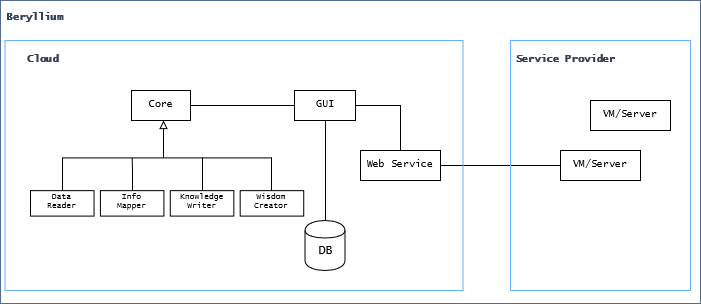
\includegraphics[width=0.8\textwidth ]{figures/analisi1.png}
        \caption [Architettura ad alto livello del sistema Beryllium]{ Architettura ad alto livello del sistema Beryllium \label{fig:architetturasitema}}
\end{figure}

Il sistema \emph{Beryllium} è composto da due principali ambienti applicativi: il \emph{cloud} e il \emph{service provider}.
\subsubsection{\underline{Cloud}}
Nell’ambiente Netcom, il \emph{Core} e la \emph{GUI} hanno un ruolo fondamentale all’interno dell’intero sistema.
La \emph{GUI} è l’interfaccia web che permette ad ogni \emph{service provider} di monitorare l'utilizzo del \emph{software} Microsoft di ogni suo cliente, gestire i contratti SPLA e generare i \emph{report} mensili.
Il \emph{Core} riceve i dati grezzi e li aggrega e manipola allo scopo di renderli fruibili all'utente finale attraverso la \emph{GUI}.
Il \emph{Core} si suddivide in ulteriori quattro componenti che elaborano i dati grezzi usando diverse modalità:
\begin{itemize}
    \item \emph{Data Reader}: legge in maniera schedulata i dati salvati nel \emph{File System} riportati dal \emph{service provider} tramite gli agenti installati e li inserisce nel \emph{database};
    \item \emph{Info Mapper}: legge i dati inseriti nel \emph{database} dal \emph{Data Reader} e li elabora opportunamente trasformandoli in oggetti;
    \item \emph{Knowledge Writer}: esegue il \emph{merge} tra gli oggetti creati dall’\emph{Info Mapper}, ottenendo così degli oggetti customizzati e mostrandoli come entità persistenti nel \emph{database}; 
    \item \emph{Wisdom Creator}: contiene l'intelligenza in grado manipolare gli oggetti customizzati e ne calcola lo SPLA.
\end{itemize}

\subsubsection{\underline{Service Provider}}

Nell’ambiente in cui opera il \emph{service provider} è necessario che ci sia almeno un \emph{server} in cui è installato il \emph{software} \emph{HypervisorScannerServices}, il quale interroga il \emph{software} che gestisce l’infrastruttura virtuale e riceve una mappa che fornisce una visione ad alto livello delle macchine e del relativo stato. La mappa dell’infrastruttura permette di conoscere la disposizione delle macchine virtuali installate e rileva e riporta eventuali spostamenti che potrebbero essere significativi per il calcolo del costo di alcune particolari licenze. Sulle macchine virtuali e fisiche di ogni \emph{service provider} è installato l’agente, il quale estrae informazioni specifiche sul \emph{server}, per quanto concerne la componente \emph{hardware}, e sui programmi Microsoft per quanto riguarda la componente \emph{software}.

\subsection{Analisi della componente Beryllium Data Collector}

Il \emph{Data Collector} è un servizio di Windows che in maniera ciclica raccoglie tutti i dati grezzi che possono essere significativi per determinare il \emph{licensing} dei prodotti Microsoft supportati.

L’architettura ad alto livello del \emph{Beryllium Data Collector} è così strutturata: 
\begin{figure}[H]
    \centering
    \captionsetup{justification=centering,margin=2cm}
        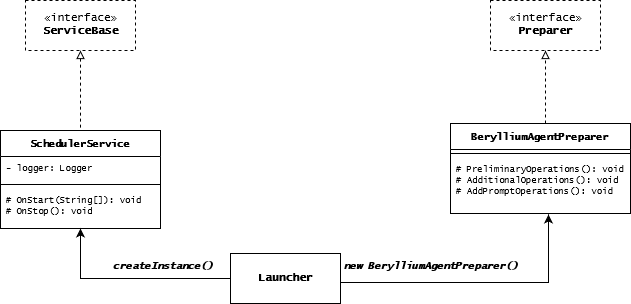
\includegraphics[width=0.8\textwidth ]{figures/analisi2.png}
        \caption [Architettura Beryllium Data Collector]{Architettura Beryllium Data Collector \label{fig:architetturadatacollector}}
\end{figure}

Ogni qualvolta che viene avviato un servizio Microsoft, viene eseguito il metodo \emph{OnStart(string[] args)}, il quale crea un nuovo \emph{thread} che invoca i metodi \emph{ScanTask()} e \emph{CheckForUpdateTask()}. In particolare:
\begin{itemize}
    \item \emph{ScanTask()}: esegue il controllo delle \emph{features} da scansionare ciclando tutte le DLL e richiamando su ognuna di esse un metodo che verifica se la feature in questione è installata nell’host dove sta operando l’agente e in caso positivo si ne estrae le informazioni;
    \item \emph{CheckForUpdateTask()}: si aggiorna se ci sono modifiche di versione
    L’agente interroga il \gl{web service} utilizzando una specifica \gl{API} a cui viene passato come parametro la versione attuale del \emph{web service}. Finita la procedura che prevede la ricerca dei dati aggiornati nel \emph{database}, le informazioni raccolte vengono aggregate in una cartella compressa. Tale cartella, che contiene i futuri \emph{file} di configurazione del \emph{Data Collector} e un eseguibile, costituisce il parametro di ritorno dell’API;
    \item \emph{CheckForUpdateTask()} esegue il \emph{file} \emph{selfUpdate.exe}, che in caso di modifiche di versione, aggiorna i \emph{file} vecchi.
\end{itemize}
L'agente è stato progettato per essere modulare in modo tale che, per supportare un nuovo prodotto Microsoft, sia sufficiente aggiungere una DLL in una \emph{directory} dell'agente.
Questa scelta progettuale presenta i seguenti principali vantaggi:
\begin{itemize}
    \item Rispetto del \gl{Single Responsibility Principle}: ogni \emph{\emph{feature}} ha un solo scopo e questo scopo è perseguito solamente da tale \emph{features};
    \item Rispetto dell’\gl{Open-Close Principle}: l’aggiunta di una nuova feature non implica nessuna modifica al codice già esistente;
    \item Riuso di codice: le DLL contengono codice utile a più di una classe e possono essere chiamata da più classi;
    \item Efficienza: le DLL non necessitano di essere salvate in RAM poiché è possibile invocarle ed eseguirle a \emph{run-time} solo quando necessario.
\end{itemize}

\subsection{Analisi di una feature del Data Collector}

Una \emph{feature} del \emph{Data Collector} si occupa di estrarre dati significativi dai prodotti Microsoft.
L’architettura di una generica \emph{feature} concreta è così strutturata:

\begin{figure}[H]
    \centering
    \captionsetup{justification=centering,margin=2cm}
        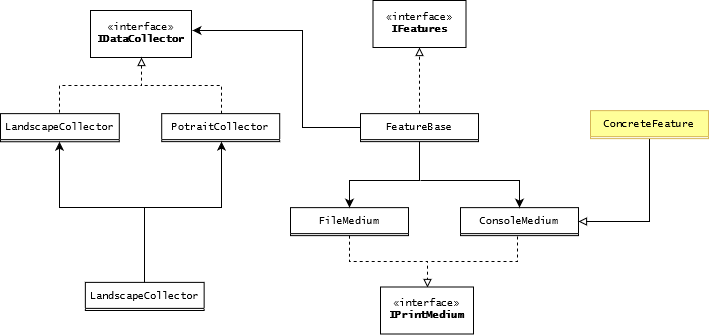
\includegraphics[width=0.7\textwidth ]{figures/analisi3.png}
        \caption [Architettura di una feature del Data Collector]{Architettura di una generica feature del Data Collector \label{fig:architetturadatacollector}}
\end{figure}

Ogni classe concreta derivata da \emph{FeatureBase} implementa i metodi astratti della classe base e ha la possibilità di definire dei metodi aggiuntivi per progettazione e funzionalità della particolare \emph{feature}. Sono presenti due modalità di raccolta dei dati che permettono di applicare un’adeguata disposizione formale ai dati raccolti. Per realizzare i due \emph{collector} è stato utilizzato il \emph{pattern} architetturale \gl{Factory} in modo da poter definire il comportamento generale e delegare alla specifica sottoclasse la costruzione del relativo oggetto. La scelta di utilizzare questo \emph{pattern creazionale} è conseguente ad un’analisi del dominio applicativo, che nello specifico caso ha ritenuto conveniente preferire un approccio che persegue la massima astrazione, piuttosto che investire sull’estendibilità della classe base.
Il \emph{Factory} viola l’\emph{Open-Close Principle}, ma in questa particolare situazione tale principio risulta poco significativo dato che è assai improbabile che ci sia la necessità di aggiungere una nuova classe concreta che implementa un terzo tipo di raccolta. \cite{pattern}
\subsubsection{\underline{Descrizione delle classi}}
Nel seguente elenco è presente una breve descrizione delle classi coinvolte nell’esecuzione di una \emph{feature}:
\begin{itemize}
    \item \emph{IDataCollector}: interfaccia contenente i metodi basilari per una generica struttura di raccolta dei dati;
    \item \emph{LandscapeCollector}: classe che raccoglie i dati in forma tabulare;
    \item \emph{PotraitCollector}: classe che raccoglie i dati in forma \emph{key-definition};
    \item \emph{DataCollectorFactory}: classe che fornisce l’istanza corretta del data collector a seconda la forma in cui i dati devono essere raccolti;
    \item \emph{IFeatures}: interfaccia contenente i metodi basilari che verranno implementati dalle varie \emph{features};
    \item \emph{FeatureBase}: classe astratta contenente i metodi comuni a tutte le \emph{features};
    \item \emph{ConcreteFeature}: classe concreta che legge e raccoglie i dati richiesti da una \emph{feature};
    \item \emph{IPrintMedium}: interfaccia contenente i metodi basilari di stampa da implementare nelle sottoclassi;
    \item \emph{FileMedium}: classe che stampa i dati su \emph{file};
    \item \emph{ConsoleMedium}: classe che stampa i dati su console.
\end{itemize}

\subsection{Analisi del Licensing Microsoft Dynamics CRM in SPLA}
I \emph{service provider} che offrono alle aziende \emph{software} Microsoft sono soggetti a un particolare programma di \emph{licensing} chiamato Service Provider Level Agreement, che prevede che ogni \emph{service provider} paghi a Microsoft un corrispettivo mensile che varia in base all'utilizzo effettivo del \emph{software} da parte dei vari clienti.
\emph{Microsoft Dynamics} CRM è un \emph{software} soggetto a SPLA utilizzato come strumento di gestione delle relazioni con i clienti e contribuisce all' automazione delle attività attraverso l’ottimizzazione delle vendite, del marketing e dell’ organizzazione di servizi.
Prendendo in considerazione il caso d'interesse, \emph{Microsoft Dynamics} CRM 2016, essendo soggetto al programma SPLA, fa riferimento allo SPUR (Service Provider Usage Rights), il documento che definisce come un \emph{service provider} può utilizzare i prodotti Microsoft.
Lo SPUR a cui fare riferimento può variare a seconda se il cliente, al momento dell’adozione del \emph{software} \emph{Microsoft Dynamics} CRM, possiede già una licenza Microsoft.
In particolare, si considera lo SPUR 2016 se il cliente ha già acquistato precedentemente una licenza compatibile, mentre si fa rifermento allo SPUR correntemente in vigore (nel nostro caso quello del 2018) se il cliente non possiede alcuna licenza al momento dell’adozione di Microsoft. \cite{microsoft-spur}
\\
Una delle opzioni di \emph{licensing} Microsoft riguardante \emph{software} soggetti ad un modello a sottoscrizione è la SAL (\emph{Subscriber Access Licens}). 
Al variare dell’utilizzo del \emph{software} \emph{Microsoft Dynamics} CRM vengono applicate diverse opzioni di SAL, mentre per quanto riguarda l’accesso di utenti esterni tramite qualsiasi applicazione o GUI, il cliente non
necessita di alcuna SAL.
Nella succesiva tabella vengono indicate le tipologie di SAL a cui sono soggetti gli utenti. \cite{microsoft-sal}
\begin{table}[H]
\newcolumntype{a}{>{\columncolor{aliceblue}}c}
\begin{tabularx}{\textwidth}{|a|X|}
	\hline
	\textbf{Essential SAL} & \textbf{Permette l’accesso al server per un utilizzo essenziale} \\\hline
	\textbf{Basic SAL} & \textbf{Permette l’accesso al server per un utilizzo di base} \\
    \hline
    \textbf{Professional SAL} & \textbf{Permette di installare e utilizzare Unified Service Desk (USD). Il permesso
di utilizzare USD è limitato agli utenti a cui sono state assegnate le SALs.} \\ \hline 
   
\end{tabularx}
    \caption {Riepilogo tipologie Subscriber Access License (SAL) \label{fig:tableSAL}}	
\end{table}

%forse inserire tabella use rights

\subsection{Requisiti}
Durante l'attività di Analisi sono stati formalizzati i requisiti. In pratica, è stata redatta una lista dettagliata e completa di tutte le caratteristiche che dovrà soddisfare il prodotto \emph{software}. 
Allo scopo di ottenere un prodotto di qualità è necessaria una rigorosa definizione dei requisiti dello stesso, in modo da avere una panoramica delle funzionalità e determinare i vincoli di qualità a cui il prodotto deve sottostare. \\
I requisiti si suddividono nelle seguenti 4 tipologie: \begin{itemize}
    \item Funzionali: descrivono una specifica funzionalità che il prodotto deve offrire;
    \item Di vincolo: indicano delle limitazioni a cui il prodotto deve sottostare;
    \item Qualitativi: indicano gli elementi atti ad aumentare la qualità del prodotto finale;
    \item Prestazionali: definiscono le performance che il prodotto deve raggiungere.
\end{itemize}

I requisiti sono stati classificati seguendo la seguente codifica:
\begin{center}
ID Requisito: R \{Categoria\} \{Priorità\}
\_ \{Codice\}
\end{center}
\begin{itemize}
    \item Categoria: indica la tipologia del requisito:
        \begin{itemize}
            \item F: Funzionale;
            \item Q: Qualitativo;
            \item P: Prestazionale;
            \item V: di Vincolo.
        \end{itemize}
        \item Priorità: ogni requisito può essere:
        \begin{itemize}
            \item Ob: obbligatorio;
            \item De: desiderabile;
            \item Fa: facoltativo;
            \item Codice: rappresenta univocamente un requisito all’interno di una categoria.
        \end{itemize}
        \item Codice: rappresenta un numero progressivo che permette di identificare univocamente un requisito all’interno di una categoria.
\end{itemize}

\begin{table}[H]
\newcolumntype{Z}[0]{>{\centering\arraybackslash}X}
\begin{tabularx}{\textwidth}{|Z|X|}
	\hline
	    \rowcolor{aliceblue}
	\textbf{ID} & \textbf{Descrizione} \\\hline
	\textbf{RFOb\_0} & \textbf{Identificare la versione di \emph{Microsoft Dynamics} CRM installata} \\
    \hline
    	\textbf{RFOb\_1} & \textbf{Estrarre informazioni solo se la versione di \emph{Microsoft Dynamics} CRM è la 2016} \\
    \hline
    	\textbf{RFOb\_2} & \textbf{Identificare le operazioni effettuate da ogni utente in una specifica data} \\
    \hline
    	\textbf{RFOb\_3} & \textbf{Distinguere le 3 tipologie di utenti (Essential, Basic, Professional)} \\
    \hline
    	\textbf{RFOb\_4} & \textbf{Individuare la modalità di scrittura corretta nel file CSV} \\
    \hline
    	\textbf{RFOb\_5} & \textbf{Analizzare i dati di \emph{audit} solo se la modalità è attiva} \\
    \hline
        	\textbf{RFOb\_6} & \textbf{Stampare i dati su file CSV} \\
    \hline
        	\textbf{RVOb\_0} & \textbf{Essere scritta in linguaggio C\#} \\
        	\hline
	    \textbf{RVOb\_1} & \textbf{Essere compilabile con .NET framework 4} \\
    \hline
	    \textbf{RVOb\_2} & \textbf{Eventuali librerie esterne utilizzate devono essere compatibili con .NET framework} \\
    \hline
    \textbf{RVOb\_3} & \textbf{Eventuali librerie esterne utilizzate devono essere compatibili con .NET framework} \\
    \hline   
    \textbf{RVDe\_0} & \textbf{La soluzione non deve richiedere l’installazione di \emph{tool} aggiuntivi sul server del cliente} \\
    \hline 
    \textbf{RVDe\_1} & \textbf{La soluzione deve essere retrocompatibile con la maggior parte diversioni di \emph{Microsoft Dynamics} CRM} \\
    \hline 
\end{tabularx}
    \caption {Tabella riassuntiva dei requisiti individuati \label{fig:requisiti}}	
\end{table}

\section{Progettazione}

Nel corso dell'attività di Progettazione, viene definito il modo in cui i requisiti individuati saranno soddisfatti.
Un'attenta attività di Progettazione prevede la definizione precisa di tutto ciò che deve essere implementato con la codifica in modo tale che, con quest’ultima attività, ci si possa focalizzare sulla scrittura del codice. 
In un primo momento è stata definita la progettazione architetturale, che definisce la struttura macroscopica del sistema con i suoi moduli e le relazioni tra di essi. Successivamente è stata costruita la progettazione di dettaglio che definisce ogni particolare delle componenti.
\\

Dopo uno studio dettagliato di \emph{Microsoft Dynamics} CRM e delle sue molteplici funzionalità, sono state individuate diverse possibilità progettuali tenendo conto di:
\begin{itemize}
    \item Vincoli di compatibilità teconologica e di versione;
    \item Retrocompatibilità;
    \item Carico di autoformazione previsto.
\end{itemize}
Dovendo progettare una DLL, il cui collegamento con l'eseguibile avviene durante l'esecuzione tramite una specifica API, che accetta in input il nome della libreria e carica all'interno dello spazio di memoria dell'applicazione la DLL sviluppata, le soluzioni prese in considerazione, si basano sulla necessità di sviluppare la libreria in C\#, come specificato nel RVOb\_0. 
     \begin{figure}[H]
        \centering
        \captionsetup{justification=centering,margin=2cm}
            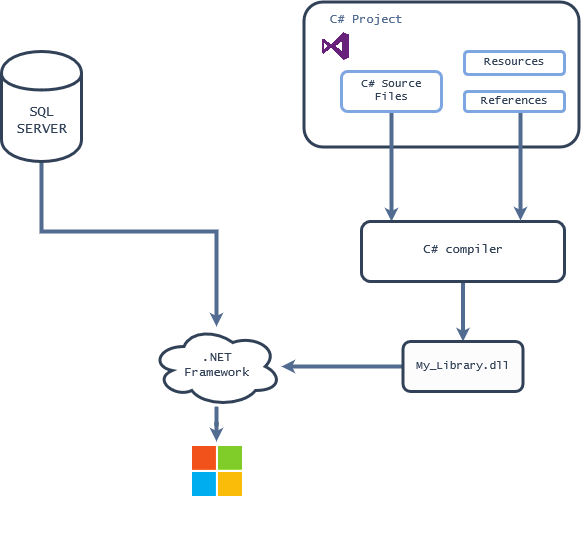
\includegraphics[width=0.6\textwidth ]{figures/powershellarch.png}
            \caption [Funzionamento dll in un progetto C\#]{Funzionamento dll in un progetto C\#\label{fig:dllfunzione}}
    \end{figure}
\subsection{Script in PowerShell}
La prima soluzione individuata prevede l’implementazione di uno \emph{script.cs1} da integrare al codice C\# che viene eseguito ogni qualvolta che viene invocata la funzione che si occupa di raccogliere i dati grezzi.
Andando a sviluppare una DLL che necessita di estrarre dati e identificare versioni è risulta più semplice usare i comandi di PowerShell rispetto al tentativo di collegarsi a tutte le classi .NET.
Lo script in questione necessita dell’importazione del modulo 
\texttt{Microsoft.Crm.PowerShell} con lo scopo di poter utilizzare il comando
\texttt{Get-CrmAccessLicense}. Il comando citato restituisce quantità
e tipologia di licenze SAL assegnate agli utenti del sistema.
Purtroppo questo comando non fornisce dati certi sull’ utilizzo del \emph{software} e delle \emph{features}.
A confermare questo dubbio sono stati eseguiti dei test da interfaccia grafica i cui risultati hanno confermato che l'assegnazione di un particolare tipo di SAL non influenza e non limita le funzionalità del prodotto.
Pertanto questa soluzione non fornisce dati attendibili sull'utilizzo effettivo del \emph{software} e il suo impiego come unica tecnologia per la raccolta dei dati va escluso.
Tuttavia le informazioni restituite dal comando \texttt{Get-CrmAccessLicense} si possono rivelare utili a posteriori, dopo aver raccolto ed elaborato i dati di utilizzo effettivi, per confrontare i risultati ottenuti dalle due soluzioni e segnalare eventuali incongruenze.
\subsection{Altre valutazioni progettuali}
Dopo aver scartato l’utilizzo esclusivo di PowerShell, sono state individuate e valutate ulteriori possibilità progettuali.
\subsubsection{\underline{Microsoft Dynamics CRM 2016 SDK}}

Microsoft mette a disposizione degli sviluppatori di \emph{Microsoft Dynamics} CRM 2016 delle \gl{SDK}, ovvero un insieme di strumenti per lo sviluppo e la documentazione del \emph{software} disponibili come pacchetti \gl{NuGet} che è possibile utilizzare nei progetti di \emph{Visual Studio}. 
\\
In particolare è stata valutata la possibilità di utilizzare il \emph{package assembly} \texttt{Microsoft.Xrm.} \\ \texttt{Tooling.Connector}, in quanto offre classi e interfacce che semplificano l'estrazione di dati dal \emph{software}.
Tuttavia il \emph{package} non rispetta il requisito di vincolo RVOb\_1, poichè necessita di essere compilato con una versione di .NET uguale o superiore alla versione 4.6.2.
\begin{figure}[H]
\centering
\captionsetup{justification=centering,margin=2cm}
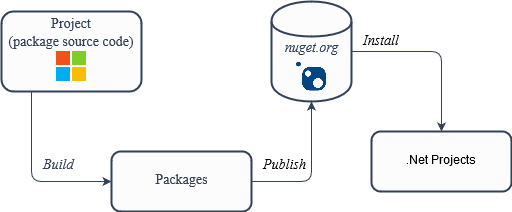
\includegraphics[width=0.6\textwidth ]{figures/sdk.png}
\caption [Funzionamento di NuGet]{Funzionamento di NuGet \label{fig:skknuget}}
\end{figure}

\subsubsection{\underline{SQL Server Reporting Services}}
\emph{SQL Server Reporting Services} (SSRS) è un generatore di \emph{report} per Microsoft e fa parte della suite di servizi di Microsoft SQL Server.
Il vantaggio di una scelta progettuale basata su questo sull'utilizzo di tale \emph{software} presenta il vantaggio di non aver bisogno di far installare all'utente nessuna applicazione aggiuntiva, dato che SSRS è un pre-requisito per l'installazione di \emph{Microsoft Dynamics} CRM. Inoltre il \emph{report} prodotto è interpretabile immediatamente da GUI.
Nonostante i vantaggi sopra elencati, la soluzione è stata scartata poiché, richiedendo una versione uguale o superiore a .NET 4.5, viola il requisito di vincolo RVOb\_1.
\subsection{Scelta finale: SQL}
Considerando rischi e benefici di ogni tecnologia, è emerso che estrarre i dati utilizzando procedure SQL risulta vantaggioso dal punto di vista implementativo e necessario rispetto ai vincoli tecnologici. 
La soluzione individuata quindi prevede la connessione al \emph{database} in cui sono salvati i dati relativi a \emph{Microsoft Dynamics} CRM e l'estrazione di metadati utili al \emph{licensing} tramite \emph{query} SQL, contenute negli appropriati metodi e classi della DLL implementata. \cite{microsoft-nuget}

\subsection{Definizione di prodotto}
La scelta progettuale individuata prevede la costruzione di due classi: \emph{DynamicsCRM} e \emph{LockPicking}.
In questo modo, è possibile separare la componente che effettua la connessione al \emph{database} ed estrae le informazioni utili, dalla componente che implementa l'interfaccia \emph{IFeature}.
Questa decisione consente di mantenere la struttura comune delle \emph{features} concrete già esistenti e delegare ad un'altra classe l'estrazione dei dati dal database.
Inoltre, alla classe concreta \emph{DynamicsCRM}, viene integrato lo script \emph{AssignedSALs}, il quale individua le SAL attualmente assegnate agli utenti e quindi fornisce i dati che verranno poi aggiunti a quelli raccolti dalla classe \emph{LockPicking}. In una fase successiva, non di competenza della studentessa, tali informazioni verranno elaborate dal core dell'applicativo, che determinerà se le SAL rilevate dallo script Powershell soddisfano quelle che corrispondono all'uso effettivo del \emph{software}.
\clearpage
\begin{figure}[H]
\centering
\captionsetup{justification=centering,margin=2cm}
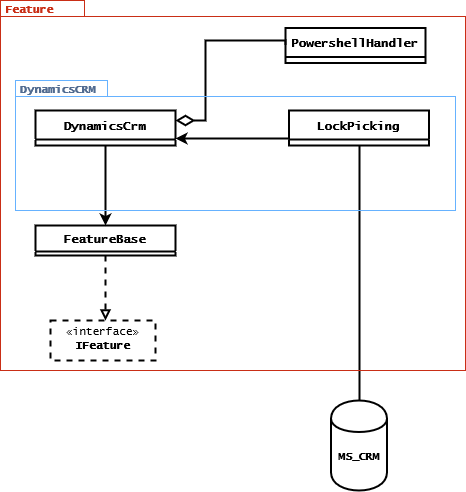
\includegraphics[width=0.6\textwidth ]{figures/CRMclassdia.png}
\caption [Diagramma delle classi della soluzione DynamicsCrm]{Diagramma delle classi della soluzione DynamicsCrm \label{fig:CRMclassDia}}
\end{figure}

La classe \emph{LockPicking} è stata progettata per aprire e chiudere la connessione al \emph{database} in cui sono salvati i dati di audit del \emph{software} \emph{Microsoft Dynamics} CRM.
Inoltre \emph{LockPicking} si occupa di interrogare il \emph{database} ed aggiungere i risultati ottenuti dalle \emph{query} al riferimento ad un oggetto di tipo \emph{DataCollector}, apposita classe dell'applicativo che permette di raccogliere dati in vari formati, passato dal costruttore della classe \emph{DynamicsCrm} al momento dell'instanziazione di un oggetto \emph{LockPicking}.
\begin{figure}[H]
\centering
\captionsetup{justification=centering,margin=2cm}
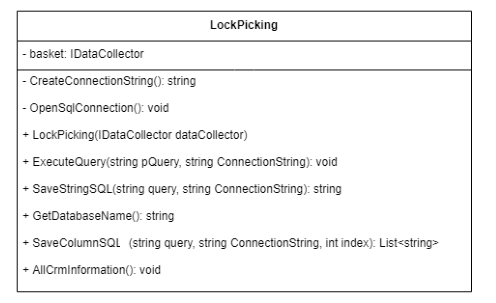
\includegraphics[width=0.6\textwidth ]{figures/lockpicking.png}
\caption [Metodi e campi della classe LockPicking]{Metodi e campi della classe LockPicking \label{fig:lockpicking}}
\end{figure}
Di seguito viene riportata una descrizione sintetica di tutti i metodi appartenenti a \emph{LockPicking}:
\begin{itemize}
    \item private readonly IDataCollector basket: data collector che raccoglie tutte le informazioni di Microsof Dynamics CRM;
    \item \textit{private static string CreateConnectionString()}: metodo che crea la \emph{connection string} per accedere al \emph{database} MS\_CRM;
    \item \textit{private static void OpenSqlConnection()}: metodo che crea la connessione con il \emph{database};
    \item \textit{public LockPicking(IDataCollector dataCollector)}: costruttore ad un parametro che istanzia un oggetto \emph{LockPicking} con il data collector opportuno;
    \item \textit{public static void ExecuteQuery(string pQuery, string ConnectionString)}: metodo che esegue una generica \emph{query};
    \item \textit{public static string SaveStringSQL(string query, string ConnectionString)}: metodo che ritorna un singolo valore di una \emph{query};
    \item \textit{public static string GetDatabaseName()}: metodo che restituisce il nome del \emph{database} nel quale è installato \emph{Dynamics} CRM;
    \item \textit{public static List<string> SaveColumnSQL(string query, string ConnectionString, int index)}: metodo che ritorna una lista di stringhe che rappresentano una colonna della tabella risultato della \emph{query};
    \item \textit{public void AllCrmInformation()}: metodo che raccoglie dati utili relativi alla \emph{feature}.
\end{itemize}
\\
La classe \emph{DynamicsCrm} implementa l'interfaccia \emph{IFeature} ed oltre all'override dei metodi della classe madre possiede il metodo proprio \emph{CheckSupportedVersion()} che serve a stabilire se la versione di \emph{Microsoft Dynamics} CRM installata è compatibile con le versioni supportate dalla soluzione. 
Inoltre tale classe, tramite l'override del metodo \emph{Gather()}, manda in esecuzione lo script Powershell e aggiunge all'oggetto \emph{DataCollector} i risultati  ottenuti dallo script in questione.
Di seguito viene riportata una descrizione sintetica di tutti i metodi e i campi appartenenti a \emph{DynamicsCrm}:
\begin{itemize}
    \item private readonly LockPicking lock\_picking; reference alla classe LockPicking;
    \item private string possibleDynamicsCRMRegistryPath: possibile percorsi nella chiave di registro per le varie versioni di Dynamics CRM;
    \item private static readonly string PS\_RESOURCE: contiene lo script Powershell da eseguire;
    \item \textit{public DynamicsCRM()}: costruttore che definisce le informazioni di base della \emph{feature};
    \item \textit{public DynamicsCRM(string pathToOutputFolder)}: costruttore completo che crea un’istanza di LockPicking;
    \item \textit{protected bool CheckSupportedVersion(string path, RegistryView view)}: metodo che verifica che la versione installata di Microsoft Dynamics CRM sia supportata dall’agente;
    \item \textit{protected void OnStepCompleted(FeatureEventArgs e)}: metodo che aggiorna il messaggio sopra la barra di avanzamento con la scritta specificata;
    \item \textit{protected void OnMessageFired(FeatureEventArgs e)}: metodo che aggiorna il messaggio sopra la barra di avanzamento con la scritta specificata e si occupa dell’avanzamento di uno step della barra;
    \item \textit{public bool IsEnabled()}: metodo verifica se \emph{Dynamics CRM} è installato sul \emph{server} \emph{Beryllium};
    \item \textit{public void Gather()}: metodo che raccoglie le informazioni.
\end{itemize}
\begin{figure}[H]
\centering
\captionsetup{justification=centering,margin=2cm}
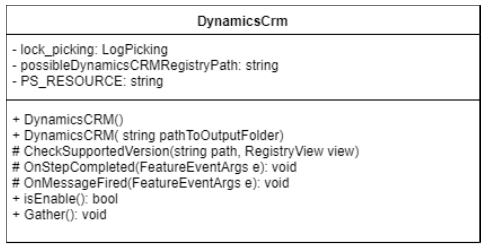
\includegraphics[width=0.6\textwidth ]{figures/dynamicscrm.png}
\caption [Metodi e campi della classe DynamicsCrm]{Metodi e campi della classe DynamicsCrm \label{fig:dynamicsCrm}}
\end{figure}

Nella seguente figura viene riportato il diagramma di sequenza che descrive le relazioni che intercorrono tra le entità del sistema nel momento in cui, dopo aver verificato che il \emph{software Microsoft Dynamics} CRM è installato sulla macchina corrente, viene avviata la procedura di estrazione dei dati al fine di produrre il documento in formato \gl{CSV} con il \emph{report} ottenuto.
\begin{figure}[H]
\centering
\captionsetup{justification=centering,margin=2cm}
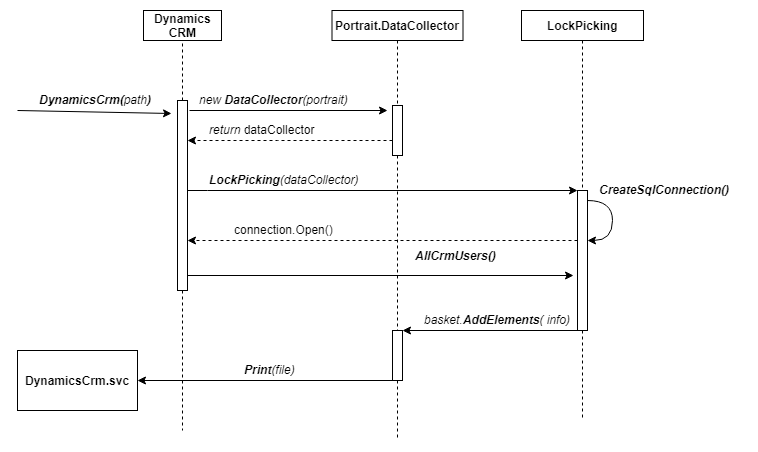
\includegraphics[width=0.9\textwidth ]{figures/sequenzaspettacolare.png}
\caption [ Diagramma di sequenza della soluzione]{ Diagramma di sequenza della soluzione \label{fig:seqdia}}
\end{figure}
\section{Codifica}
Prima di procedere alla descrizione dell'attività di codifica, è necessario precisare che il prototipo richiesto ha come scopo l’esclusiva verifica della fattibilità della feature. È stato volutamente tralasciato l’aspetto legislativo che regolamenta l’autorizzazione e l’utilizzo di dati degli utenti con la conseguente ripercussioni della privacy normata a livello europeo dalla \gl{GDPR}.
Grazie alla progettazione dettagliata e alle conoscenze pregresse di programmazione ad oggetti in Java e del linguaggio SQL, la scrittura del codice delle classi \emph{LockPicking} e \emph{DynamicsCrm} non è risultata particolarmente complessa. 
Al contrario ha richiesto più tempo del previsto implementare l'accesso e il recupero dei dati da Registro di sistema, in quanto era necessario conoscere approfonditamente il comportamento di API .NET poco documentate.\\
Per quanto riguarda lo sviluppo dello script in Powershell, pur non avendo esperienze pregresse con tale linguaggio, l'attività di codifica è risultata piuttosto agevole rispetto a quanto preventivato, dato che dispone di un set di comandi (\emph{cmdlet}) progettati per gestire oggetti e quindi concettualmente più affini alle tecniche di programmazione affrontate durante il percorso universitario. Tuttavia, pur essendo avendo una sintassi intuitiva, Powershell non fornisce strumenti di segnalazione degli errori di battitura e ciò ha reso impegnativa l'attività di debugging sullo script.\\
L'utilizzo dell'ambiente di sviluppo \emph{Visual Studio} 2016 ha semplificato significativamente la procedura di configurazione e integrazione della soluzione \emph{DynamicsCrm} al progetto già esistente. Inoltre l'IDE suggerisce automaticamente i nomi dei metodi e i tipi dei parametri richiesti relativi ai \emph{namespace} esterni utilizzati, semplificando la scrittura del codice e riducendo gli errori sintattici.
\begin{figure}[H]
\centering
\captionsetup{justification=centering,margin=2cm}
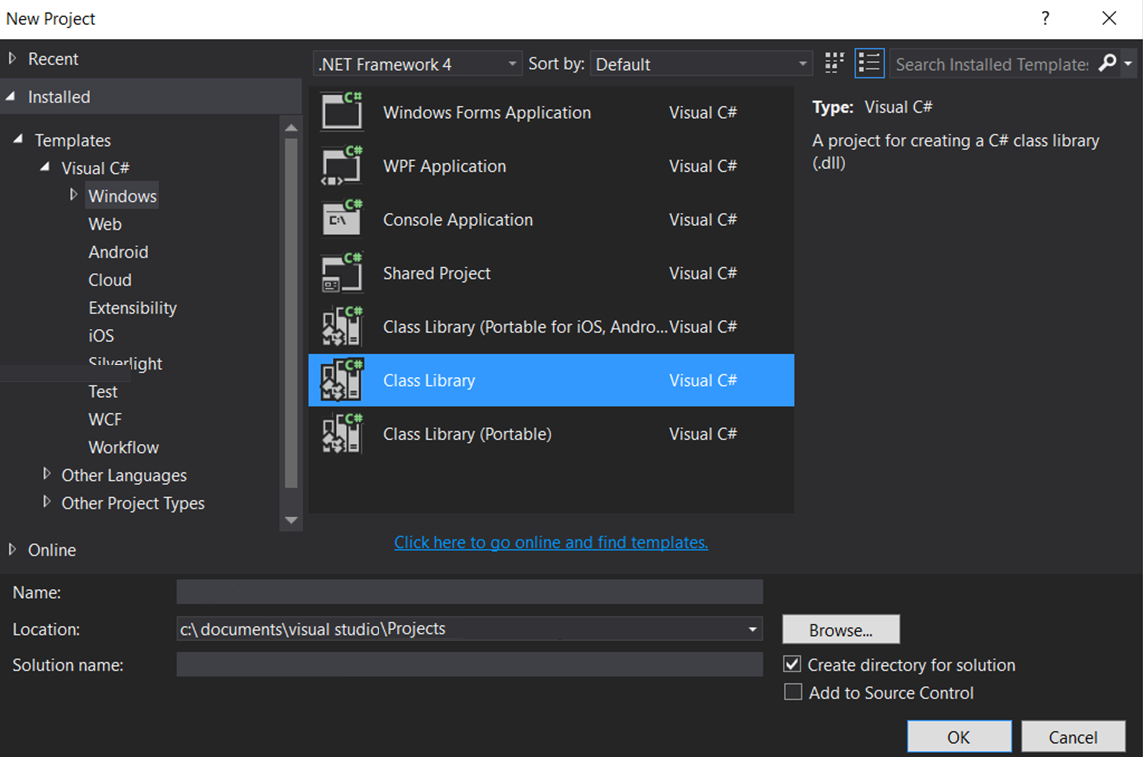
\includegraphics[width=0.7\textwidth ]{figures/dllvisual.png}
\caption [Screenshot creazione progetto DLL in Visual Studio 2016]{ Screenshot della finestra di creazione di un progetto DLL in Visual Studio 2016 \label{fig:dllvisual}}
\end{figure}
Di seguito viene riportata la struttura della directory della \emph{feature} sviluppata:
\dirtree{%
.1 DynamicsCrm.dll.
    .2 References.
    .2 Scripts.
        .3 AssignedSALs.ps1.
    .2 DynamicsCrm.csproj.
    .2 LockPicking.cs.
    .2 DynamicsCrm.cs.
}


\section{Documentazione}
L’azienda ha richiesto inoltre la produzione dei documenti di Analisi dei Requisiti e Specifica Tecnica, i quali sono stati redatti rispettivamente durante le fasi di Analisi e Progettazione.
Per la stesura della documentazione sono stati utilizzati dei \emph{template} di documentazione interni su cui si basano tutti i documenti dell’azienda.
\section{Test}
\subsection{Ambiente di test e raccolta dati}
Come previsto dal piano di lavoro, durante la fase iniziale, è stato creato e configurato l'ambiente di test. In particolare è stata implementata una macchina virtuale con sistema operativo Windows, ospitata dal \emph{server} dell'azienda, sulla quale è stato installato il \emph{software} \emph{Microsoft Dynamics} CRM 2016, dopo averne soddisfatto i dipendenze \emph{software} richiesti. 
In accordo con la metodologia aziendale, il tutor mi ha fornito una struttura \gl{Active Directory} già implementata e destinata ai test. Successivamente, accedendo all'SQL Server della macchina virtuale attraverso l'account utente avente i permessi da amministratore, utilizzando l'interfaccia grafica di \emph{Microsoft Dynamics} CRM 2016, ho assegnato ad ogni utente una tipologia di SAL diversa, in modo da avere tutte e le tipologie di licenza e dunque di coprire tutti i casi possibili. 
Quotidianamente, è stato eseguito l'accesso al prodotto utilizzando gli account dei tre utenti precedentemente individuati e per ognuno di essi sono state eseguite diverse operazioni sulle entità persistenti, in modo da avere una quantità di dati sufficienti per garantire l'attendibilità dei risultati.
\subsection{Esecuzione dei test}
Durante l'ultima settimana di stage sono state realizzate tre tipologie di test:
\begin{itemize}
    \item Test di unità; 
    \item Test di integrazione;
    \item Test di sistema.
\end{itemize}
I risultati dei test sono stati poi riportati in forma tabulare, per aumentarne la leggibilità e permetterne una rapida consultazione. 
\subsubsection{\underline{Test di unità}}
I test di unità hanno lo scopo di verificare che tutte le unità, ovvero le componenti composte da uno o più moduli elementari, funzionino correttamente.
\begin{table}[H]
%\newcolumntype{a}{>{\columncolor{aliceblue}}c}
\begin{tabularx}{\textwidth}{|c|X|c|X|}
	\hline
	\rowcolor{aliceblue}
	{ID test} & {Descrizione}  & {Esito} & {Componenti} \\ \hline
	\multirow{ 2}{*}{UT\_1} & {Si verifica che avvenga la connessione al database}  & {\textcolor{limegreen}{Superato}} & { CreateConnectionString(): string;} \\ & &  & {OpenSqlConnection(): void }  \\
	\hline
\end{tabularx}
    \caption {Esempio: Struttura della tabella per i Test di Unità \label{fig:tableUT}}	
\end{table}
\clearpage
\subsubsection{\underline{Test di Integrazione}}
Una volta svolti i test sulle unità, si può procedere con l’esecuzione dei test di integrazione, che combinano tali unità in componenti testandone la corretta integrazione.
L'approccio \gl{bottom-up} utilizzato pervede la seguente strategia d’integrazione: si sviluppano e si integrano prima le parti con minore dipendenza funzionale e maggiore utilità. In questo modo, vengono prima testati i package più semplici e con meno dipendenze, per poi procedere con una base solida per i test successivi.
\begin{table}[H]
%\newcolumntype{a}{>{\columncolor{aliceblue}}c}
\begin{tabularx}{\textwidth}{|c|X|c|X|}
	\hline
	\rowcolor{aliceblue}
	{ID test} & {Descrizione}  & {Esito} & {Componenti} \\ \hline
	{IT\_1} & {Si verifica che la corretta integrazione tra DynamicsCrm e FeaureBase}  & {\textcolor{limegreen}{Superato}} & {Features} \\
	\hline
	{IT\_2} & {Si verifica che la corretta integrazione tra DynamicsCrm e LockPicking, controllando che i risultati dei possibili flussi di dati corrispondano a quelli attesi}  & {\textcolor{limegreen}{Superato}}  & {Features.DynamicsCrm} \\ 
	\hline
\end{tabularx}
    \caption {Esempio: Struttura della tabella per i Test di Integrazione \label{fig:tableIT}}	
\end{table}

\subsubsection{\underline{Test di sistema}}
I test di sistema hanno lo scopo di verificare la copertura dei requisiti definiti durante l’attività di analisi e sono utili per prepararsi al collaudo. In particolare questi test sanciscono una versione definitiva del \emph{software} sviluppato.
\begin{table}[H]
%\newcolumntype{a}{>{\columncolor{aliceblue}}c}
\begin{tabularx}{\textwidth}{|c|X|c|c|}
	\hline
	\rowcolor{aliceblue}
	{ID test} & {Descrizione}  & {Esito} & {Requisito} \\ \hline
	{ST\_1} & {Si verifica che venga individuata la versione attesa di Microsoft Dynamics CRM installata} & {\textcolor{limegreen}{Superato}} & {RFOb\_0} \\
	\hline
	{ST\_2} & {Si verifica che vengano identificare le operazioni effettuate da ogni utente in una specifica data}  & {\textcolor{limegreen}{Superato}} & {RFOb\_2} \\
	\hline
\end{tabularx}
    \caption {Esempio: Struttura della tabella per i Test di Sistema \label{fig:tableST}}	
\end{table}

Per effettuare il collaudo finale, è stato preparato un ambiente dedicato sul \emph{server} aziendale e una volta eseguiti tutti i test, l'agente è stato eseguito dal tutor aziendale.
\begin{figure}[H]
\centering
\captionsetup{justification=centering,margin=2cm}
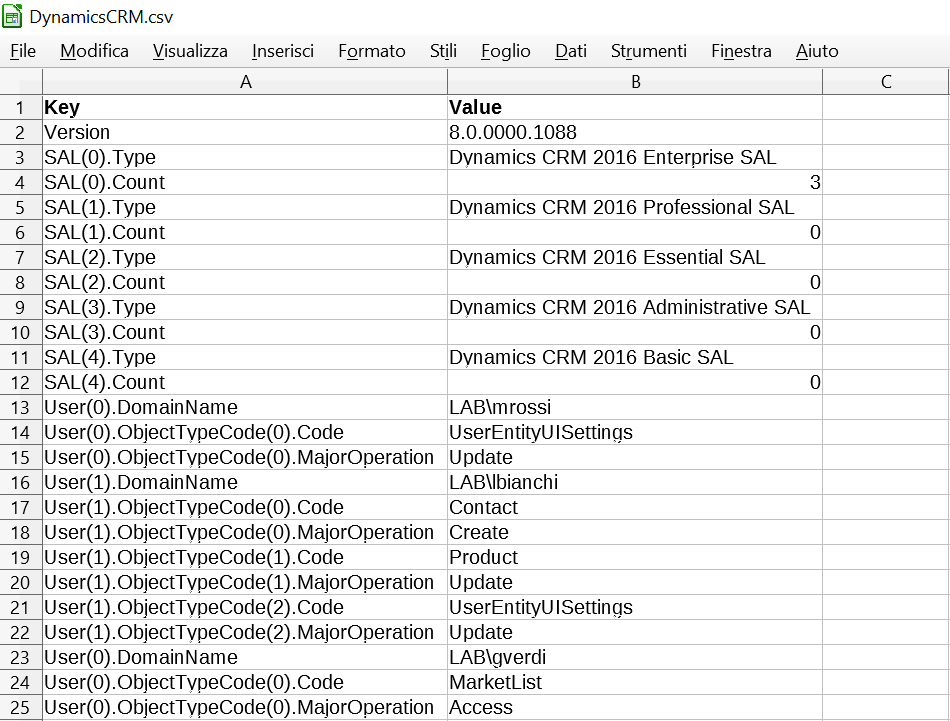
\includegraphics[width=0.9\textwidth ]{figures/output.png}
\caption [Output prodotto dall'esecuzione dell'agente in fase di collaudo]{Output prodotto dall'esecuzione dell'agente in fase di collaudo \label{fig:outputcollaudo}}
\end{figure}
%\section{Risultati finali}
